% !TeX program = pdflatex
\documentclass[11pt,a4paper]{article}
\usepackage[utf8]{inputenc}
\usepackage[T1]{fontenc}
\usepackage[turkish]{babel}
\usepackage{lmodern}
\usepackage{geometry}
\usepackage{graphicx}
\usepackage{caption}
\usepackage{subcaption}
\usepackage{booktabs}
\usepackage{siunitx}
\usepackage{hyperref}
\usepackage{longtable}
\usepackage{xcolor}
\geometry{margin=2.5cm}
\hypersetup{colorlinks=true,linkcolor=blue,citecolor=blue,urlcolor=blue}

\title{NPM Ekosisteminde Top N Paket İçin Yönlü Karmaşık Ağ Analizi: Merkeziyet, Risk Skoru ve Robustluk}
\author{\textbf{Yusuf Talha ARABACI}}
\date{\today}

\begin{document}
\maketitle

\begin{abstract}
Bu çalışma, NPM ekosistemindeki popüler Top~N paketi, bağımlılık ilişkilerine göre yönlü bir karmaşık ağ (Dependent~$\to$~Dependency) olarak modellemekte ve yapısal riskleri merkeziyet metrikleriyle incelemektedir. Veri, her çalıştırmada API'lerden (öncelikle ecosyste.ms; yedek olarak npm registry ve npms.io) çekilmektedir. Ağ, NetworkX ile kurulmakta; in-degree, out-degree ve betweenness merkeziyet metrikleri hesaplanmaktadır. Büyük grafiklerde betweenness hesaplaması örnekleme (k) ile hızlandırılmaktadır. Çalışma ayrıca bileşik bir risk skoru (normalize edilmiş in/out/between ağırlıklı toplamı) ve risk tabanlı robustluk analizi (kritik düğümlerin kaldırılması) önermektedir. Üretilen tüm çıktılar (CSV/MD/JSON ve PNG/SVG görseller) results/ dizininde saklanır.
\end{abstract}

\section{Giriş}
Yazılım tedarik zinciri saldırılarında (SSCA), tek bir bağımlılığın ele geçirilmesi geniş çapta zincirleme etkilere yol açabilir. NPM ekosistemi, yoğun bağımlılık ilişkilerine sahip olup, paketlerin yapısal konumuna göre sistemik risk taşıyabilmektedir. Bu çalışma, Top~N paket üzerinden inşa edilen yönlü bağımlılık ağı ile aşağıdaki sorulara odaklanır:
\begin{itemize}
  \item Hangi düğümler (paketler) yapısal olarak kritik (yüksek in-degree, yüksek betweenness)?
  \item Hangi düğümler geniş bağımlılık yüzeyine sahip (yüksek out-degree)?
  \item Merkeziyetlere dayalı bileşik bir risk skoru ile risk liderleri nasıl sıralanır?
  \item Kritik düğümler kaldırıldığında ağın bağlanırlığı nasıl değişir (robustluk)?
\end{itemize}

\section{\c{C}al\i\c{s}man\i n Amac\i}
Bu \c{c}al\i\c{s}man\i n temel amac\i, yaz\i l\i m tedarik zinciri g\"uvenli\u{g}ini yap\i sal bir bak\i\c{s} a\c{c}\i s\i yla yeniden tan\i mlamak ve mevcut g\"uvenlik de\u{g}erlendirme yakla\c{s}\i mlar\i na a\u{g} bilimi temelli bir \"o\l c\"ut kazand\i rmakt\i r. Geleneksel sistemler (\"or. CVSS), riski yaln\i zca paket i\c{c}i zafiyetlerle \"ol\c{c}erken; ger\c{c}ekte risk, paketin ba\u{g}\i ml\i oldu\u{g}u ve kendisine ba\u{g}\i ml\i olan paketlerle kurdu\u{g}u ili\c{s}kilerden de kaynaklan\i r. Bu nedenle NPM ekosistemindeki paketleri bir \emph{karma\c{s}\i k a\u{g}} olarak modelleyerek, her bir paketin a\u{g} i\c{c}indeki yap\i sal \"onemini, ele ge\c{c}irilmesi durumunda yaratabilece\u{g}i basamaklanma (\emph{cascading}) etkisini ve bunun sistemik g\"uvenlik riski \"uzerindeki nicel etkilerini bilimsel metriklerle \"ol\c{c}meyi ve \"ong\"ormeyi hedefliyoruz.


\section{Veri ve Yöntem}
Top~N paket listesi, her çalıştırmada API'lerden çekilir. Öncelik ecosyste.ms üzerinde indirmeye göre sıralı paket adlarındadır; başarısız durumlarda npm registry araması (popularity) ve npms.io (popülerlik skoru) yedek olarak kullanılır. Bağımlılıklar, npm registry'de paketlerin en güncel sürümlerinin \texttt{dependencies} alanından okunur; isteğe bağlı olarak \texttt{peerDependencies} de dahil edilebilir. Yönlü ağ, Dependent~$\to$~Dependency yönüyle kurulur. Büyük graflarda betweenness merkeziyeti örneklemeli (k) hesaplanır.

\section{Ağ Modeli ve Metrikler}
Model, NetworkX ile kurulmuş \texttt{DiGraph} yapısıdır. Temel metrikler:
\begin{itemize}
  \item \textbf{In-Degree:} Düğüme gelen kenar sayısı (bu pakete dayanan paket sayısı). Ele geçirilirse etki alanını gösterir.
  \item \textbf{Out-Degree:} Düğümün dış bağımlılık sayısı. Bağımlılık zinciri uzunluğu/karmaşıklığına işaret eder.
  \item \textbf{Betweenness:} En kısa yollardaki aracılık. Köprü rolünü ve tek hata noktası potansiyelini gösterir.
\end{itemize}

\section{Bulgular}
Bu bölümde, results/ dizinindeki çıktıları kullanarak görsel ve tablolu özetler sunulmaktadır.

\subsection{Ağ Görselleştirmeleri}
\begin{figure}[h]
  \centering
  \IfFileExists{network_full_topN.png}{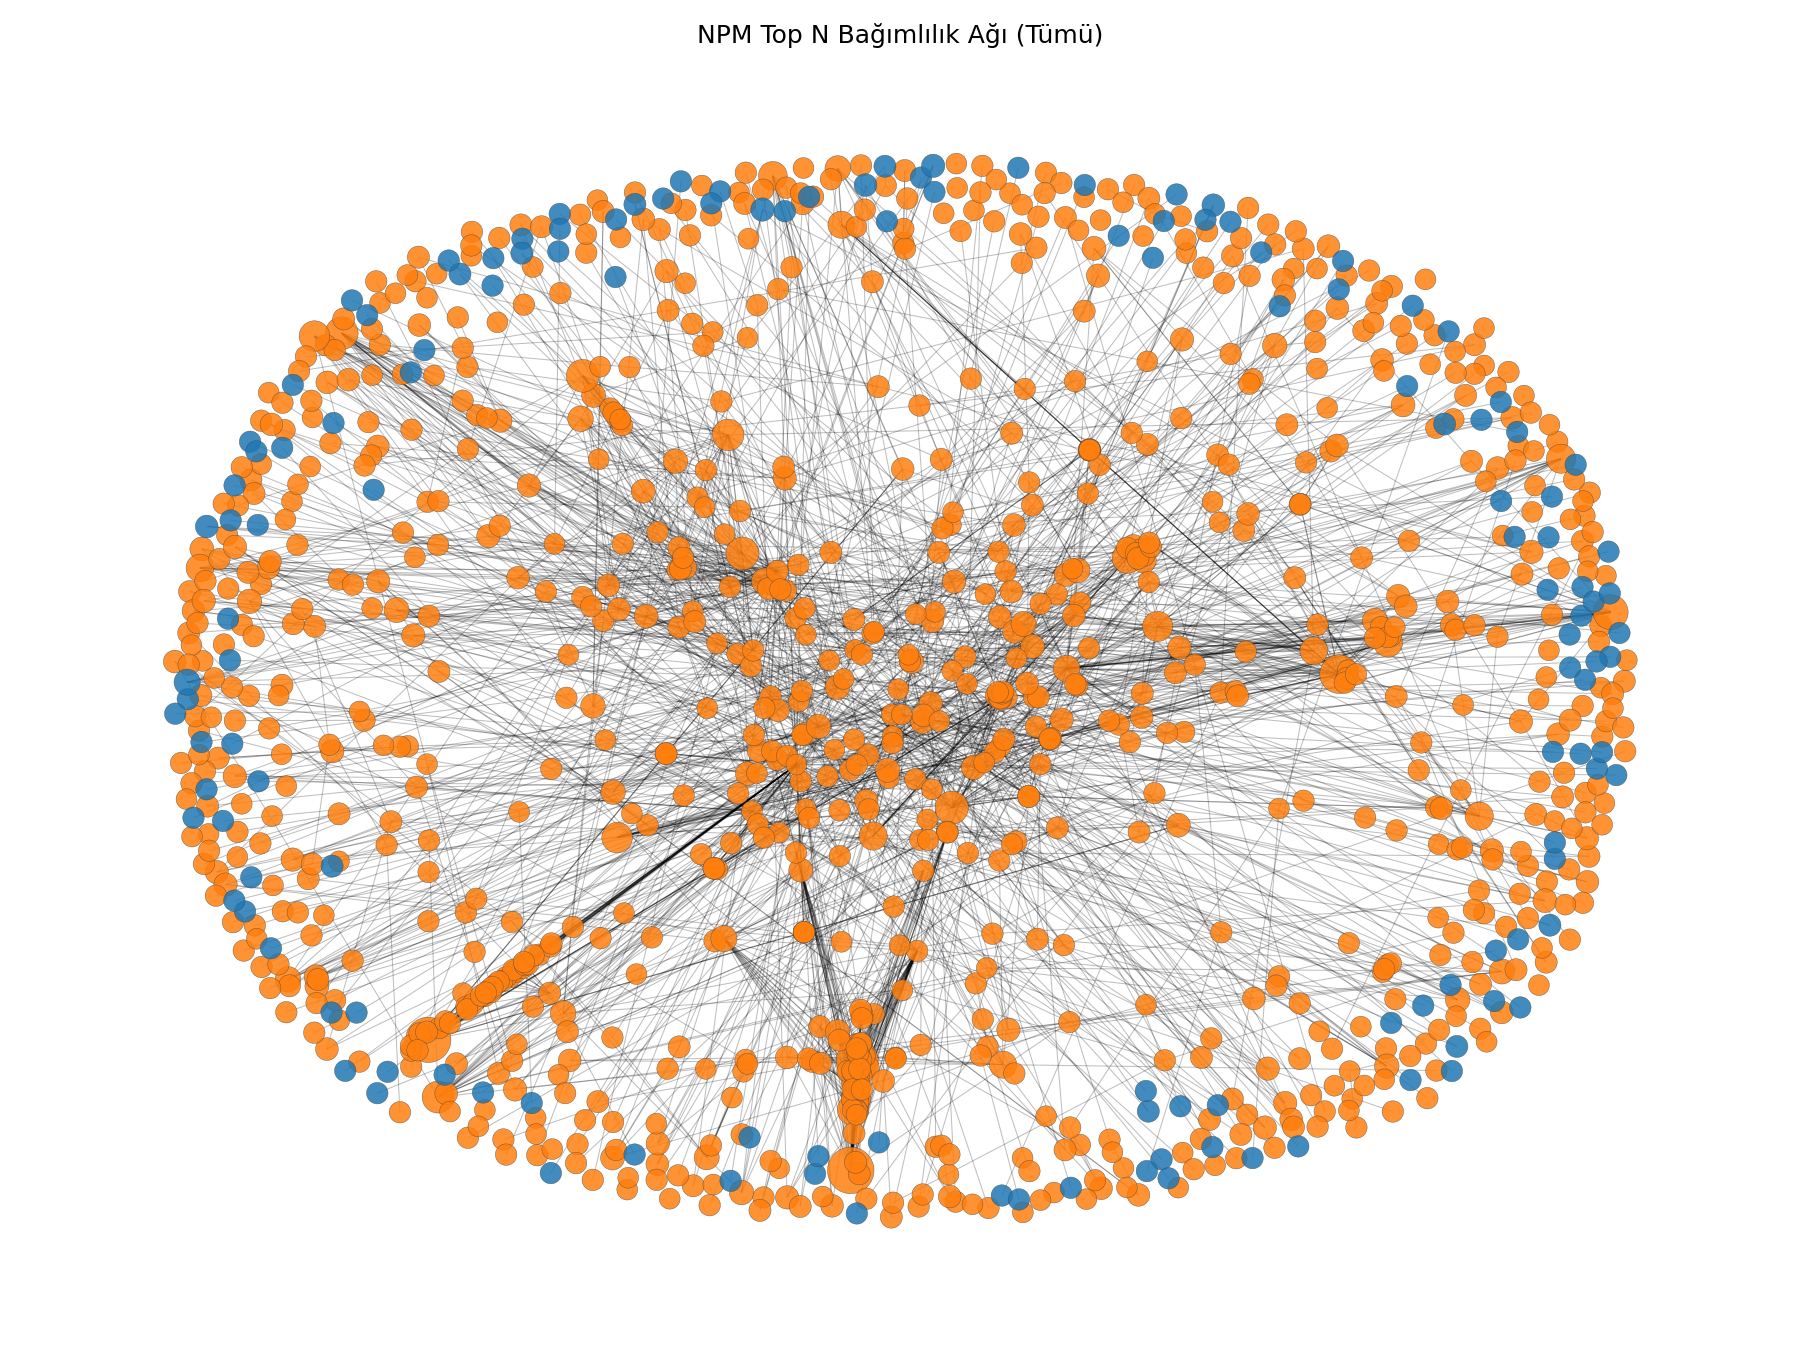
\includegraphics[width=0.95\linewidth]{../results/network_full_topN.png}}{\fbox{network\_full\_topN.png bulunamadı}}
  \caption{Top N + bağımlılıkların oluşturduğu yönlü ağ (düğüm boyutu: in-degree, renk: Top N turuncu / diğerleri mavi).}
\end{figure}

\begin{figure}[h]
  \centering
  \IfFileExists{network_topN_only.png}{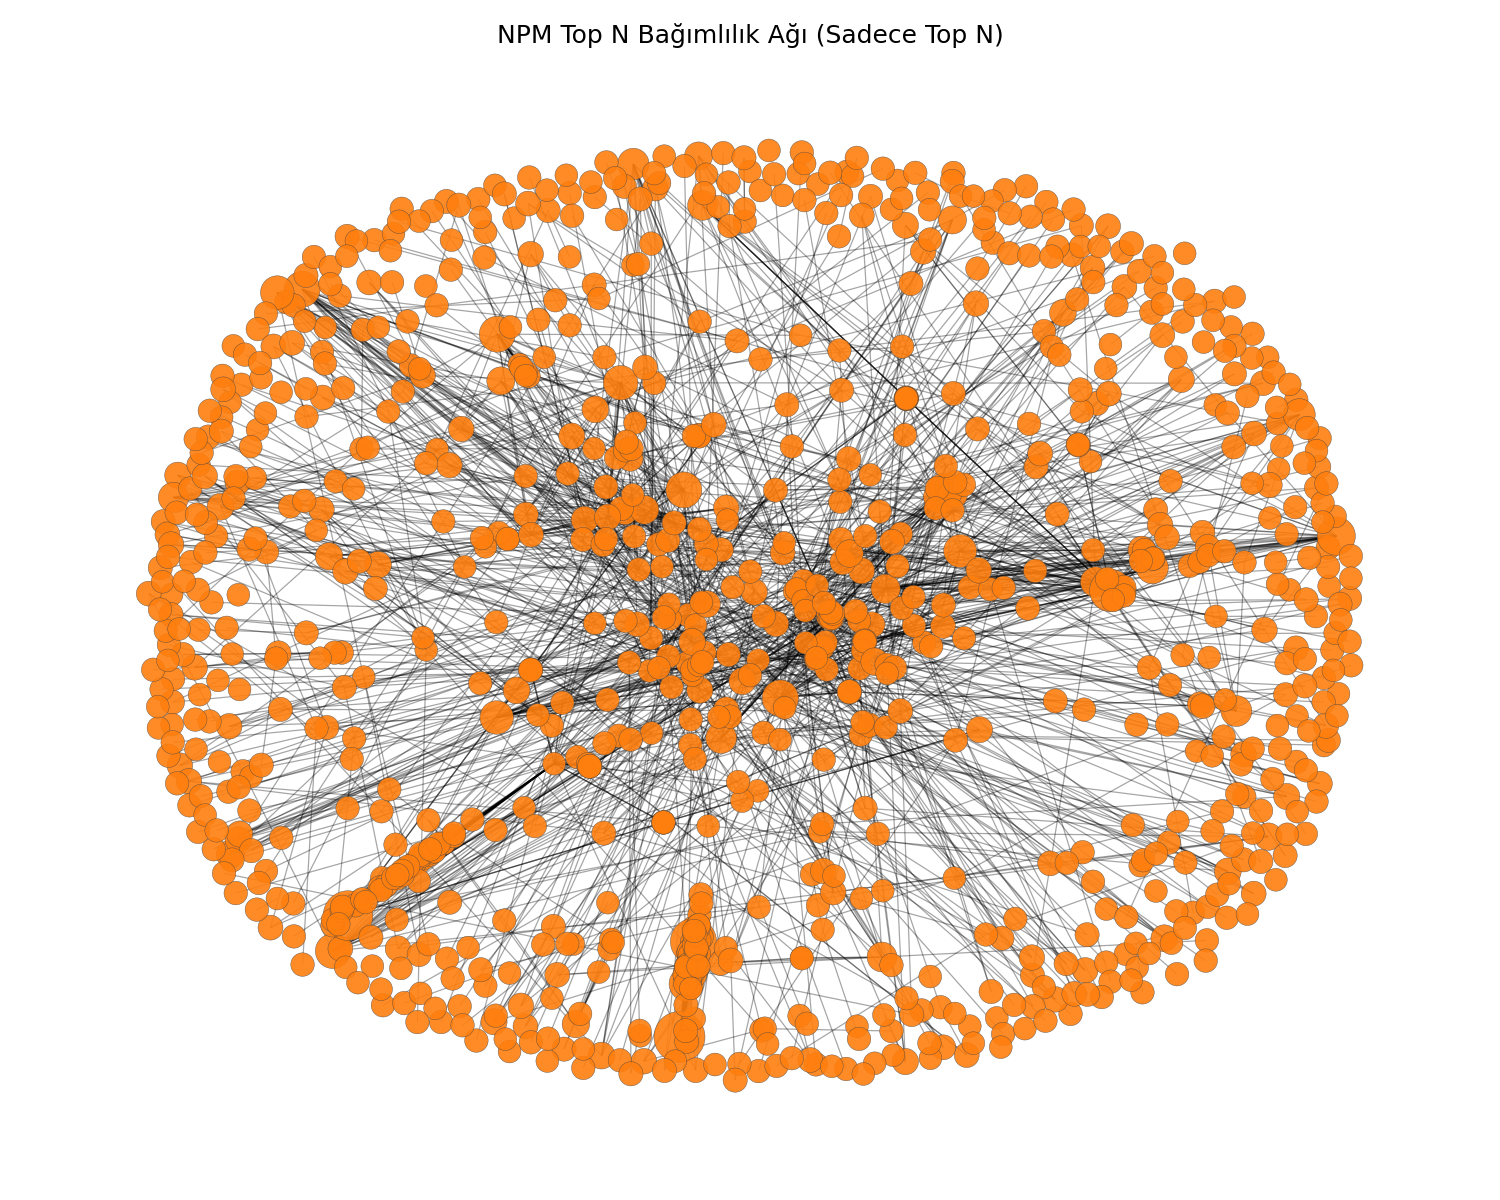
\includegraphics[width=0.85\linewidth]{../results/network_topN_only.png}}{\fbox{network\_topN\_only.png bulunamadı}}
  \caption{Sadece Top N düğümlerin indüklenmiş alt-ağı.}
\end{figure}

\subsection{Derece Dağılımları ve Korelasyonlar}
\begin{figure}[h]
  \centering
  \IfFileExists{degree_histograms.png}{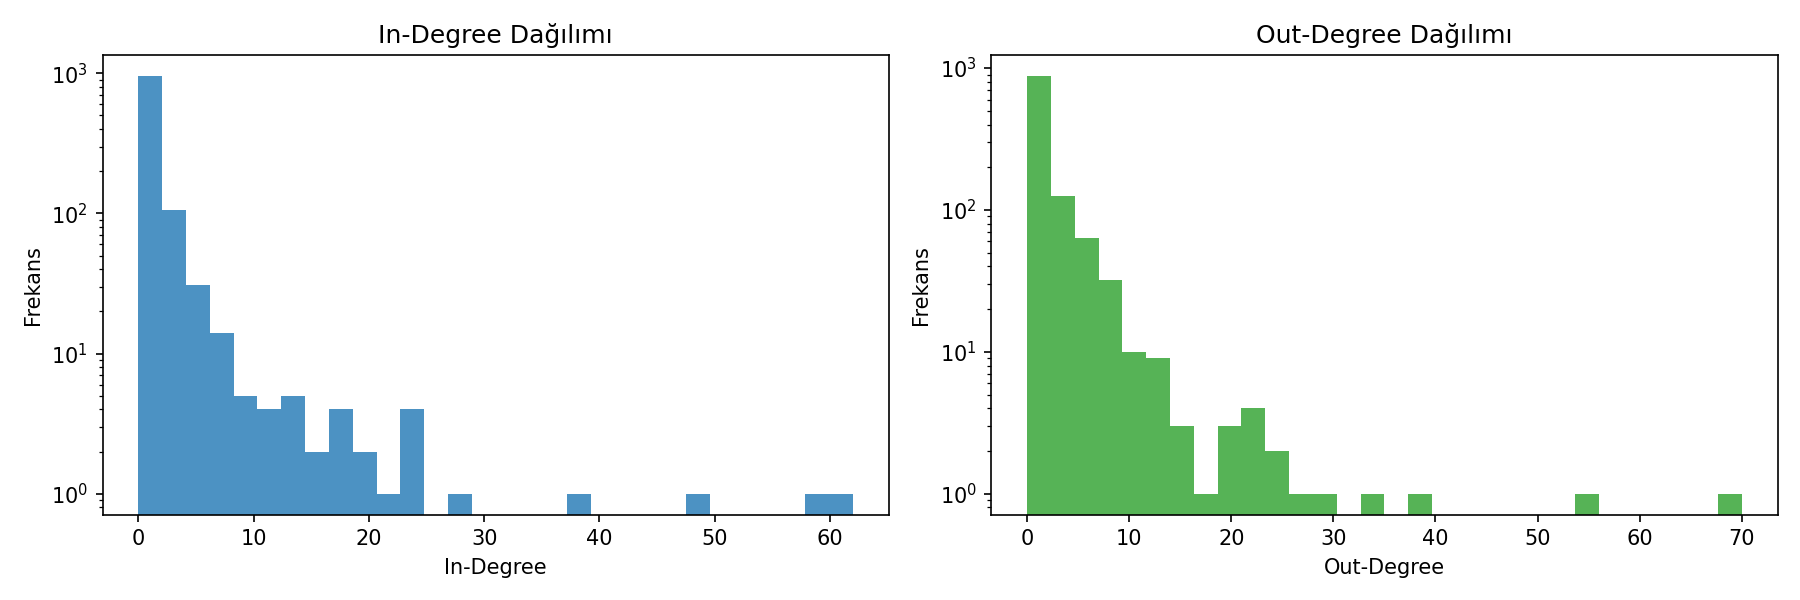
\includegraphics[width=0.95\linewidth]{../results/degree_histograms.png}}{\fbox{degree\_histograms.png bulunamadı}}
  \caption{In-Degree ve Out-Degree histogramları (log ölçek).}
\end{figure}

\begin{figure}[h]
  \centering
  \IfFileExists{scatter_correlations.png}{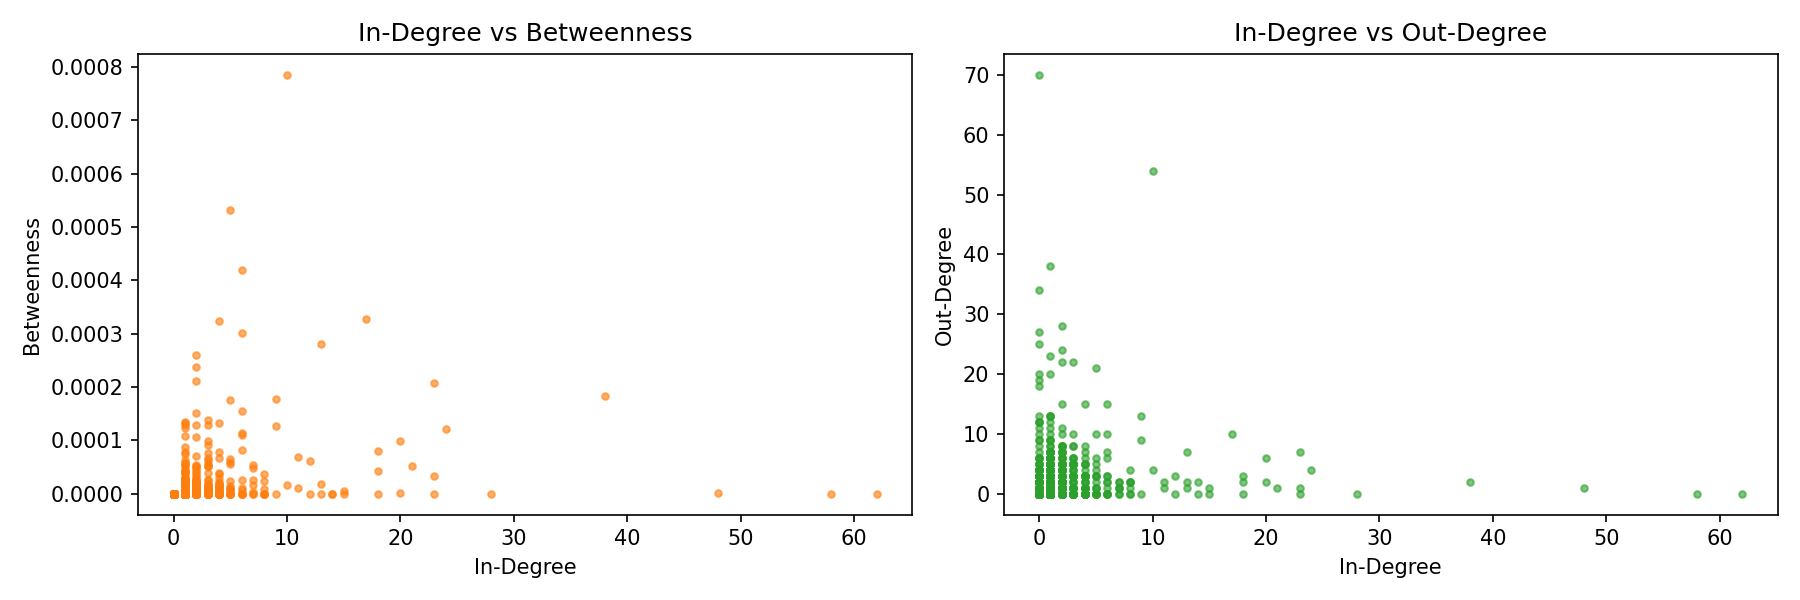
\includegraphics[width=0.95\linewidth]{../results/scatter_correlations.png}}{\fbox{scatter\_correlations.png bulunamadı}}
  \caption{Korelasyonlar: In-Degree vs Betweenness (solda), In-Degree vs Out-Degree (sağda).}
\end{figure}

\subsection{Liderler (İlk 10)}
\begin{figure}[h]
  \centering
  \IfFileExists{top10_leaders.png}{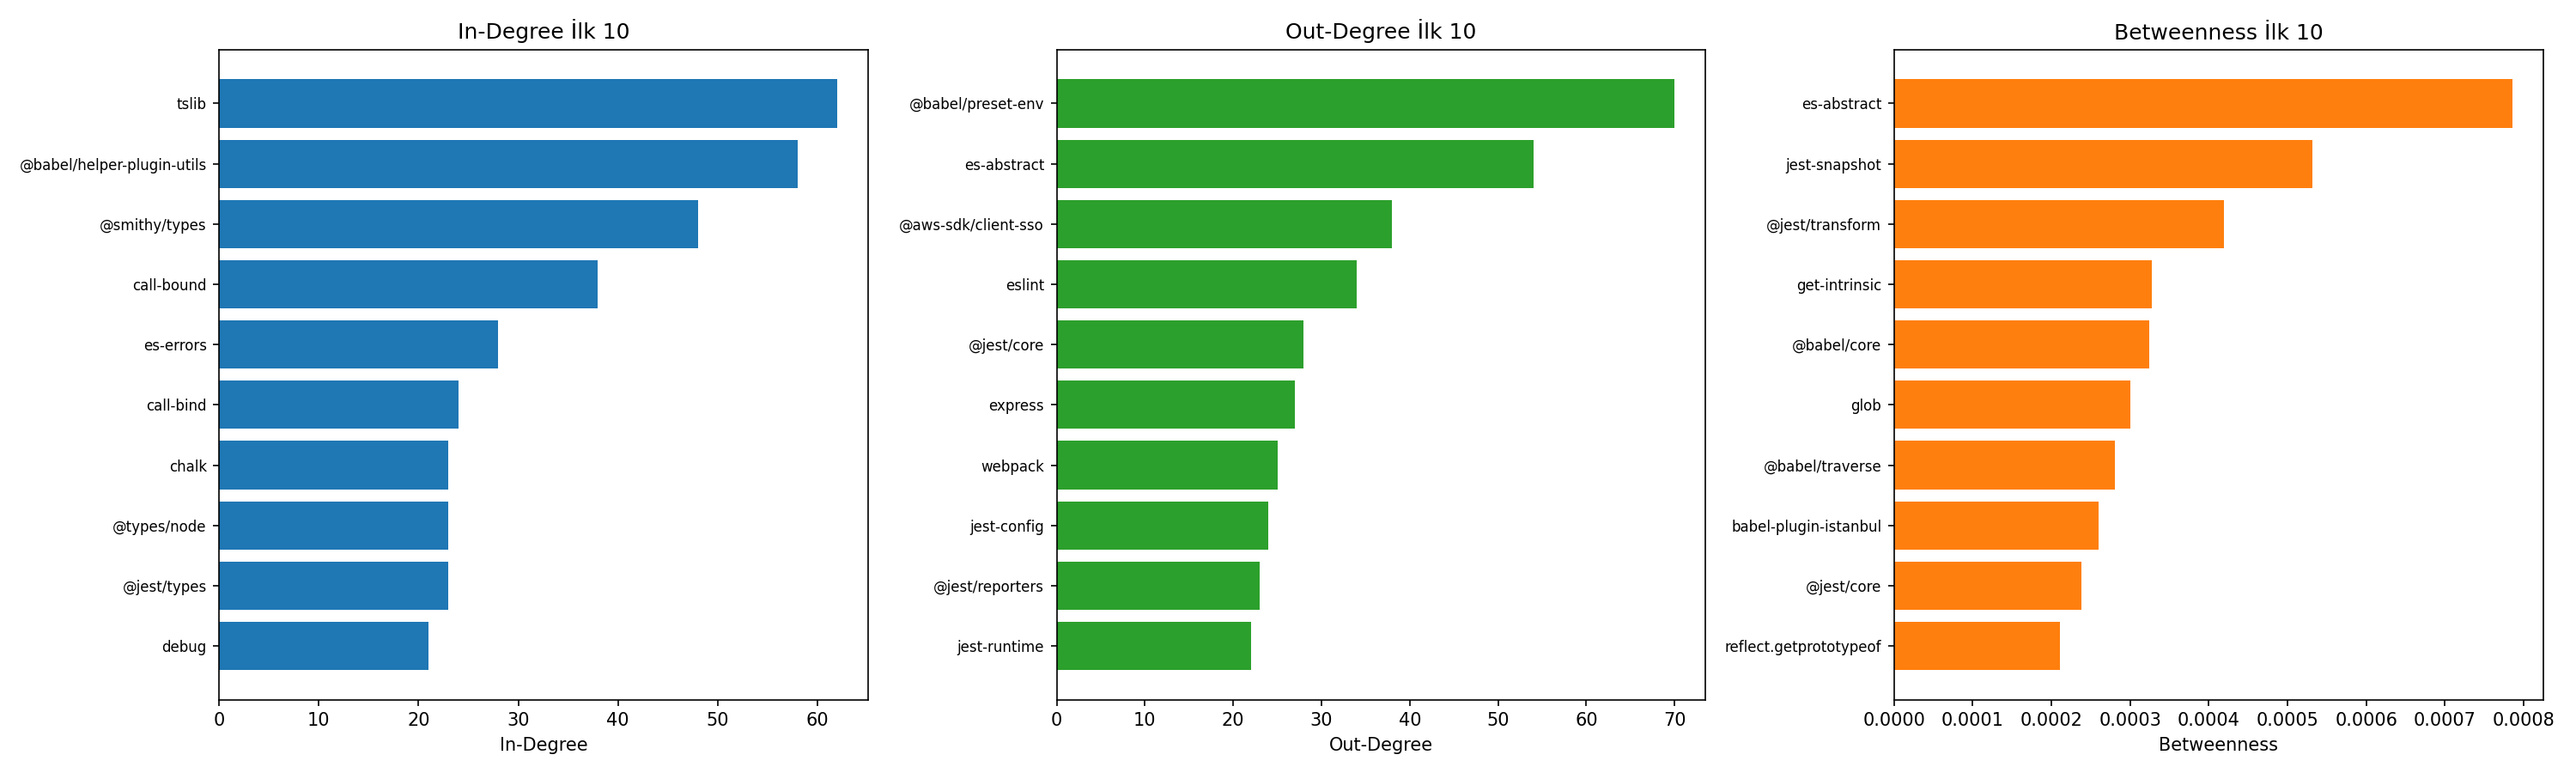
\includegraphics[width=0.95\linewidth]{../results/top10_leaders.png}}{\fbox{top10\_leaders.png bulunamadı}}
  \caption{İlk 10 lider (In/Out-Degree ve Betweenness).}
\end{figure}

\subsection{Ek Görseller}
\begin{figure}[h]
  \centering
  \IfFileExists{top10_in_degree.png}{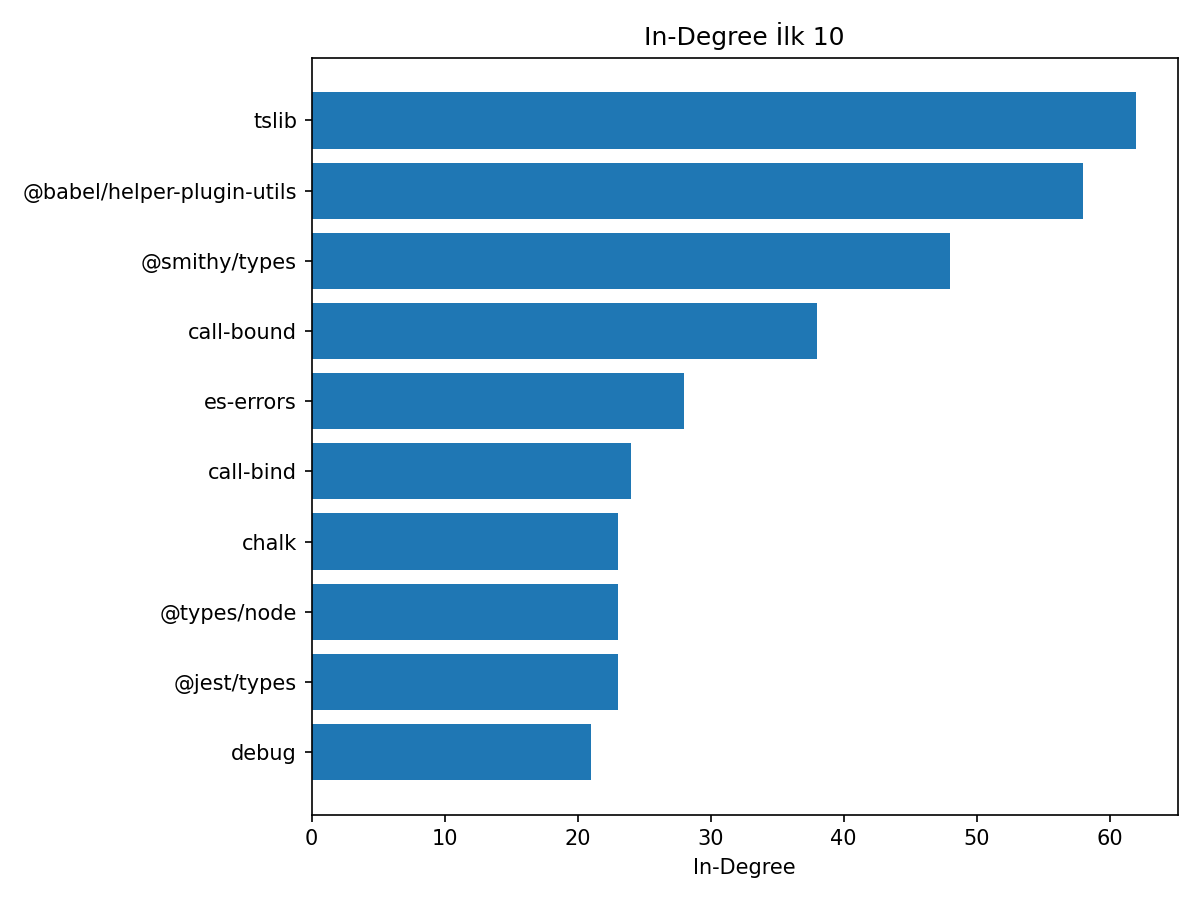
\includegraphics[width=0.48\linewidth]{../results/top10_in_degree.png}}{\fbox{top10\_in\_degree.png yok}}
  \IfFileExists{top10_out_degree.png}{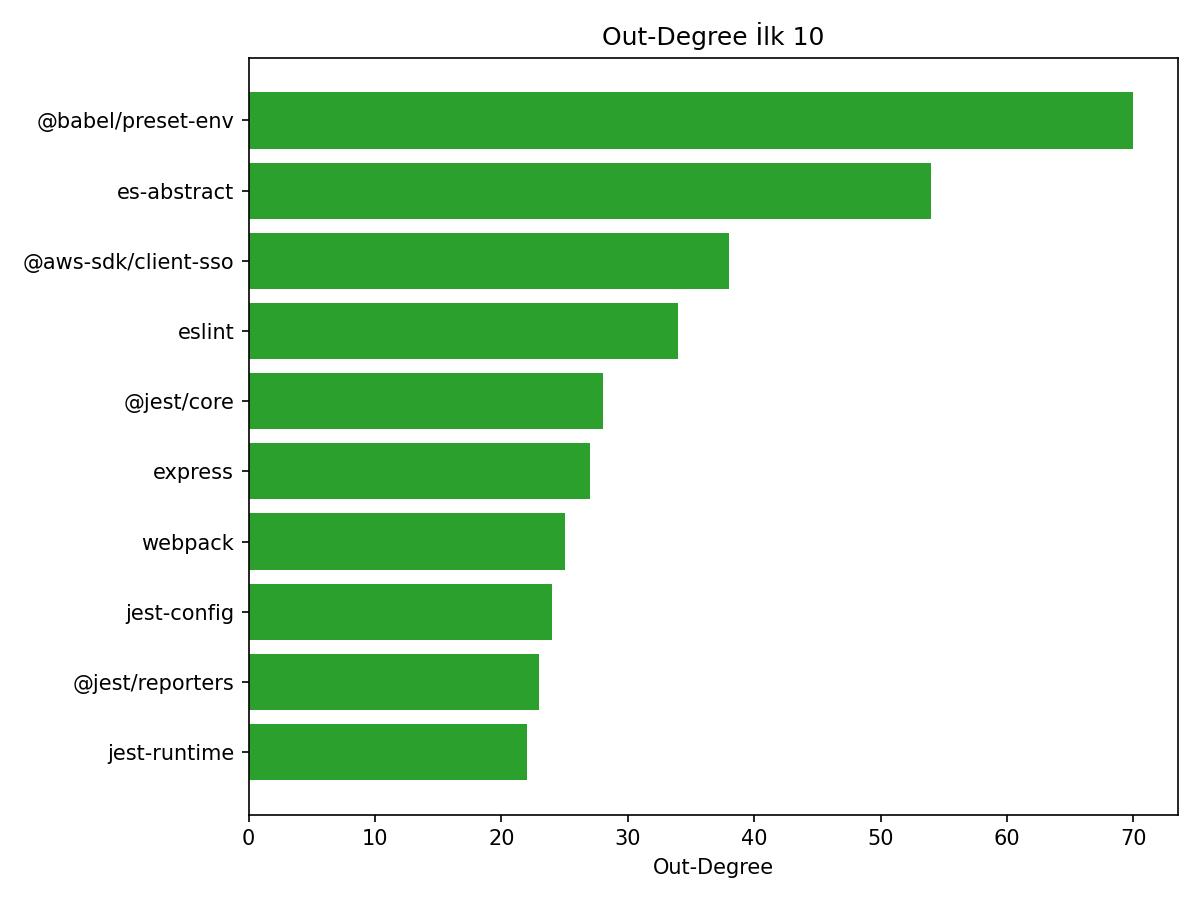
\includegraphics[width=0.48\linewidth]{../results/top10_out_degree.png}}{\fbox{top10\_out\_degree.png yok}}
  \caption{İlk 10 In-Degree (sol) ve Out-Degree (sağ).}
\end{figure}

\begin{figure}[h]
  \centering
  \IfFileExists{top10_betweenness.png}{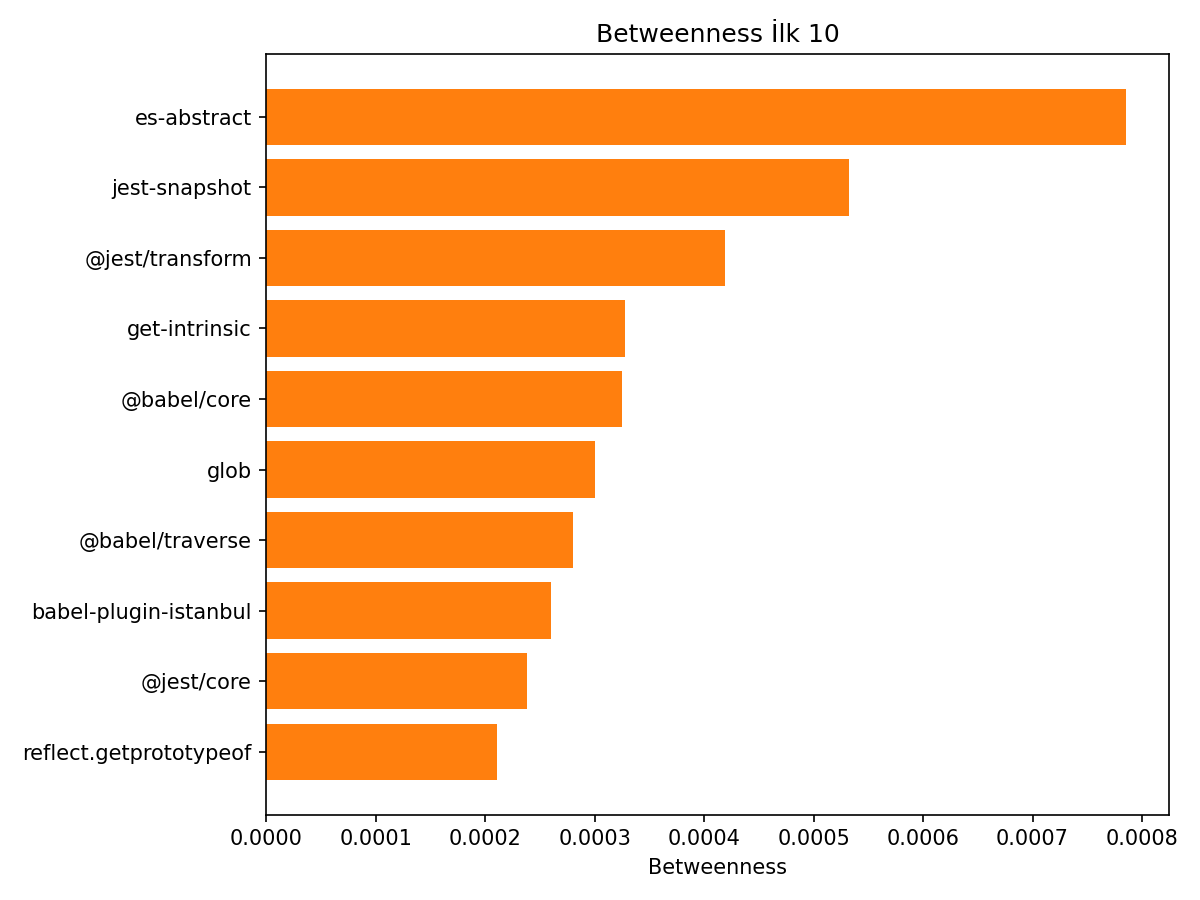
\includegraphics[width=0.6\linewidth]{../results/top10_betweenness.png}}{\fbox{top10\_betweenness.png yok}}
  \caption{İlk 10 Betweenness.}
\end{figure}

\subsection{Risk Skoru ve Robustluk}
\begin{figure}[h]
  \centering
  \IfFileExists{top20_risk.png}{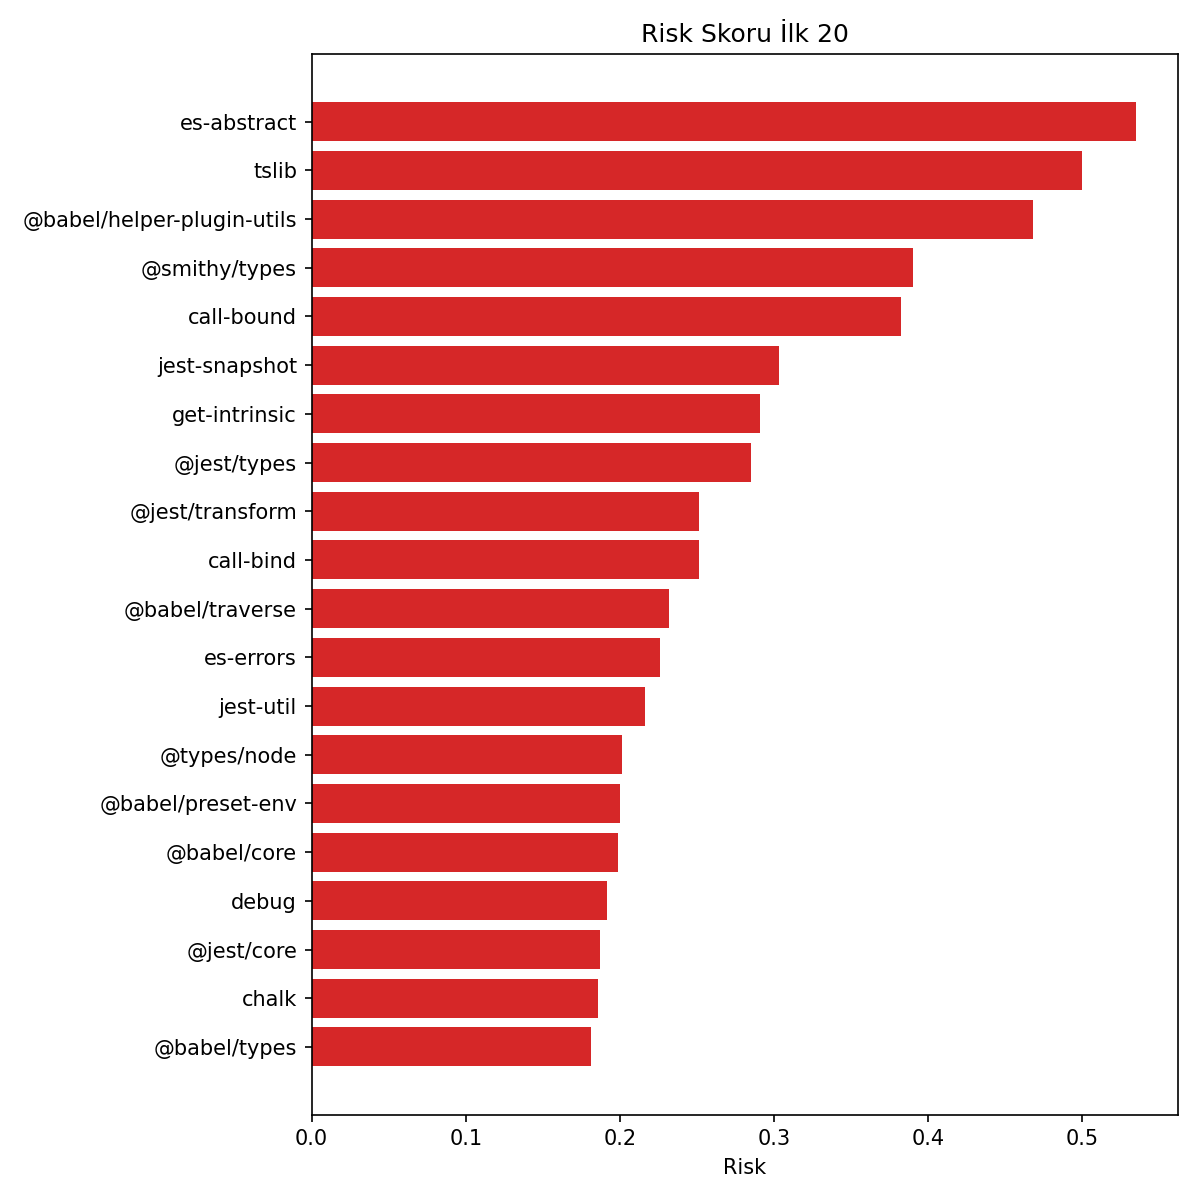
\includegraphics[width=0.75\linewidth]{../results/top20_risk.png}}{\fbox{top20\_risk.png bulunamadı}}
  \caption{Bileşik risk skoruna göre ilk 20 paket.}
\end{figure}

\paragraph{Edge Betweenness İlk 10.} Aşağıdaki tablo, en yüksek edge betweenness değerine sahip 10 kenarı göstermektedir.


\subsection{Ek Tablolar}
\paragraph{Top 20 In-Degree (Tüm Düğümler).}
\IfFileExists{../results/metrics_top20_in_degree.tex}{\begin{table}[h]
\centering
\\\caption{Top 20 In-Degree (Toplam Düğümler)}
\begin{tabular}{lrrrr}
\toprule
Paket & In-Degree & Out-Degree & Betweenness & TopN? \\ \midrule
tslib & 62 & 0 & 0.000000 & True \\
@babel/helper-plugin-utils & 58 & 0 & 0.000000 & True \\
@smithy/types & 48 & 1 & 0.000001 & True \\
call-bound & 38 & 2 & 0.000183 & True \\
es-errors & 28 & 0 & 0.000000 & True \\
call-bind & 24 & 4 & 0.000121 & True \\
@jest/types & 23 & 7 & 0.000207 & True \\
@types/node & 23 & 1 & 0.000034 & True \\
chalk & 23 & 0 & 0.000000 & True \\
debug & 21 & 1 & 0.000051 & True \\
@aws-sdk/types & 20 & 2 & 0.000002 & True \\
jest-util & 20 & 6 & 0.000099 & True \\
@babel/types & 18 & 2 & 0.000079 & True \\
define-properties & 18 & 3 & 0.000043 & True \\
graceful-fs & 18 & 0 & 0.000000 & True \\
get-intrinsic & 17 & 10 & 0.000328 & True \\
es-object-atoms & 15 & 1 & 0.000006 & True \\
gopd & 15 & 0 & 0.000000 & True \\
@smithy/protocol-http & 14 & 2 & 0.000000 & True \\
semver & 14 & 0 & 0.000000 & True \\
\bottomrule
\end{tabular}
\end{table}
}{\fbox{metrics\_top20\_in\_degree.tex bulunamadı}}

\paragraph{Top 20 Risk Skoru.}
\IfFileExists{../results/risk_scores_top20.tex}{\begin{longtable}{lrrrrr}
\caption{Top 20 Risk Skoru}\\
\toprule
Paket & Risk & In-Degree & Out-Degree & Betweenness & TopN? \\
\midrule
\endfirsthead
\toprule
Paket & Risk & In-Degree & Out-Degree & Betweenness & TopN? \\
\midrule
\endhead
\bottomrule
\endfoot
\bottomrule
\endlastfoot
es-abstract & 0.534931 & 10 & 54 & 0.000785 & True \\
tslib & 0.500000 & 62 & 0 & 0.000000 & True \\
@babel/helper-plugin-utils & 0.467742 & 58 & 0 & 0.000000 & True \\
@smithy/types & 0.390249 & 48 & 1 & 0.000001 & True \\
call-bound & 0.382129 & 38 & 2 & 0.000183 & True \\
jest-snapshot & 0.303511 & 5 & 21 & 0.000532 & True \\
get-intrinsic & 0.290993 & 17 & 10 & 0.000328 & True \\
@jest/types & 0.284735 & 23 & 7 & 0.000207 & True \\
@jest/transform & 0.251456 & 6 & 15 & 0.000419 & True \\
call-bind & 0.251171 & 24 & 4 & 0.000121 & True \\
@babel/traverse & 0.231984 & 13 & 7 & 0.000280 & True \\
es-errors & 0.225806 & 28 & 0 & 0.000000 & True \\
jest-util & 0.216164 & 20 & 6 & 0.000099 & True \\
@types/node & 0.201331 & 23 & 1 & 0.000034 & True \\
@babel/preset-env & 0.200000 & 0 & 70 & 0.000000 & True \\
@babel/core & 0.199075 & 4 & 15 & 0.000324 & True \\
debug & 0.191845 & 21 & 1 & 0.000051 & True \\
@jest/core & 0.187008 & 2 & 28 & 0.000238 & True \\
chalk & 0.185484 & 23 & 0 & 0.000000 & True \\
@babel/types & 0.181088 & 18 & 2 & 0.000079 & True \\
\end{longtable}
}{\fbox{risk\_scores\_top20.tex bulunamadı}}

\subsection{Basamaklanma (Cascading Impact)}
Bir d\"u\u{g}\u m\"un ele ge\c{c}irilmesi halinde, ters y\"onde (dependents) ula\c{s}\i labilen d\"u\u{g}\u m say\i s\i o d\"u\u{g}\u m\"un potansiyel etki alan\i n\i g\"osterir. Risk liderleri i\c{c}in hesaplanan basamaklanma etkisi a\c{s}a\u{g}\i daki g\"orsele d\"ok\"ulm\u\c{s}t\u{u}r.
\begin{figure}[h]
  \centering
  \IfFileExists{cascade_impact_top20.png}{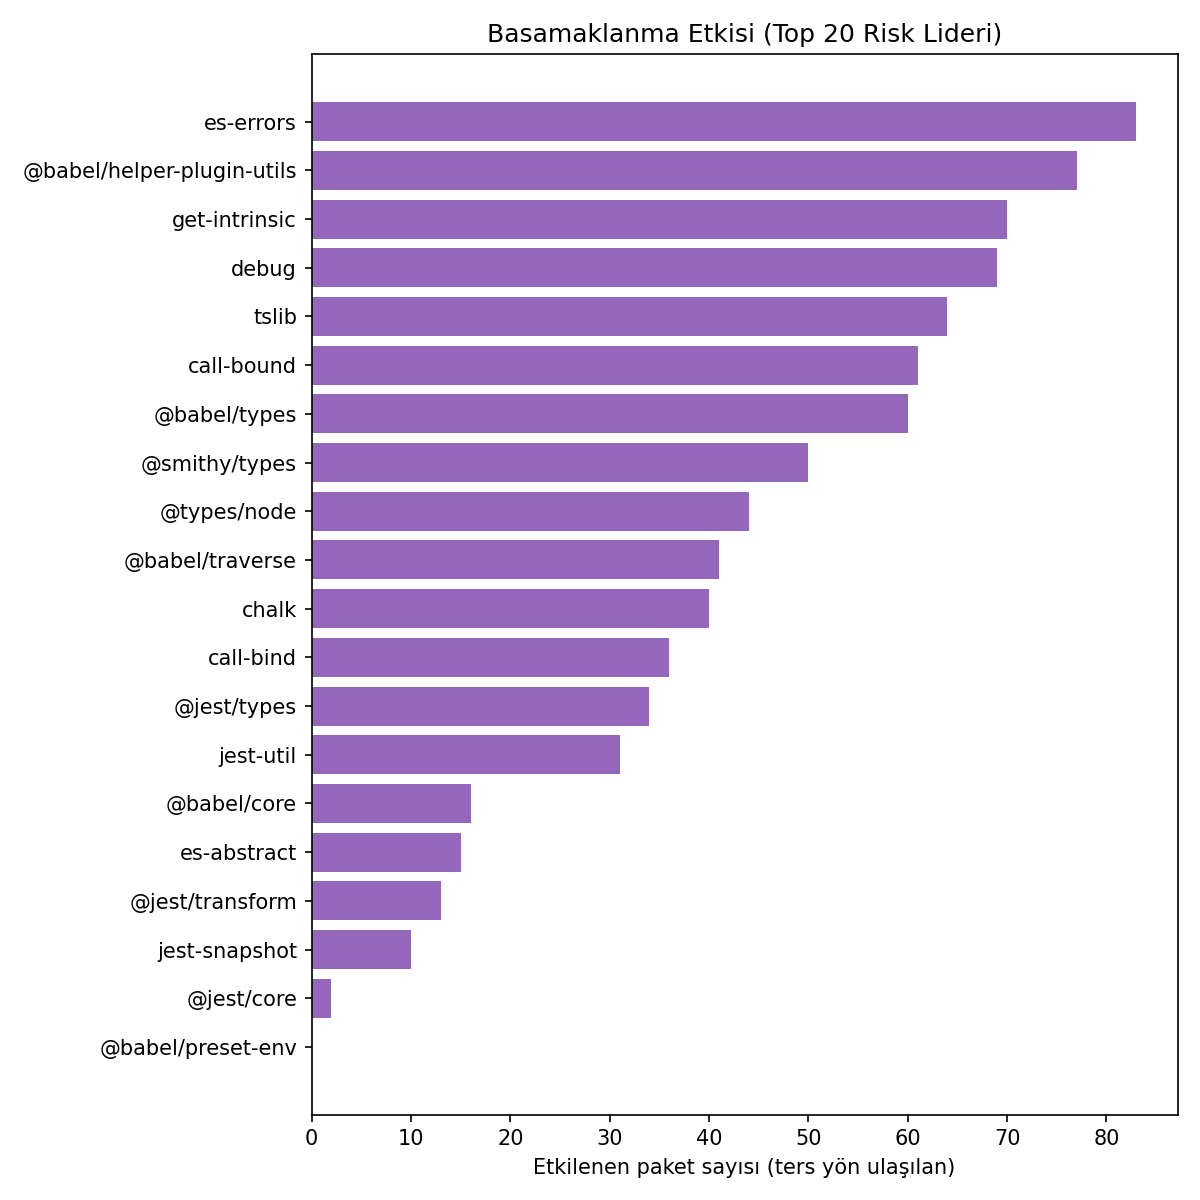
\includegraphics[width=0.75\linewidth]{../results/cascade_impact_top20.png}}{\fbox{cascade\_impact\_top20.png bulunamad\i}}
  \caption{Risk skoruna g\"ore ilk 20 paket i\c{c}in basamaklanma (cascading impact) b\"uy\"ukl\"u\u{g}\u{u}.}
\end{figure}

\paragraph{Risk--Basamaklanma \c{C}izimi.} Ek olarak, risk skoru ile basamaklanma etkisi aras\i ndaki ili\c{s}ki de g\"ozlemlenmi\c{s}tir.
\begin{figure}[h]
  \centering
  \IfFileExists{risk_vs_cascade.png}{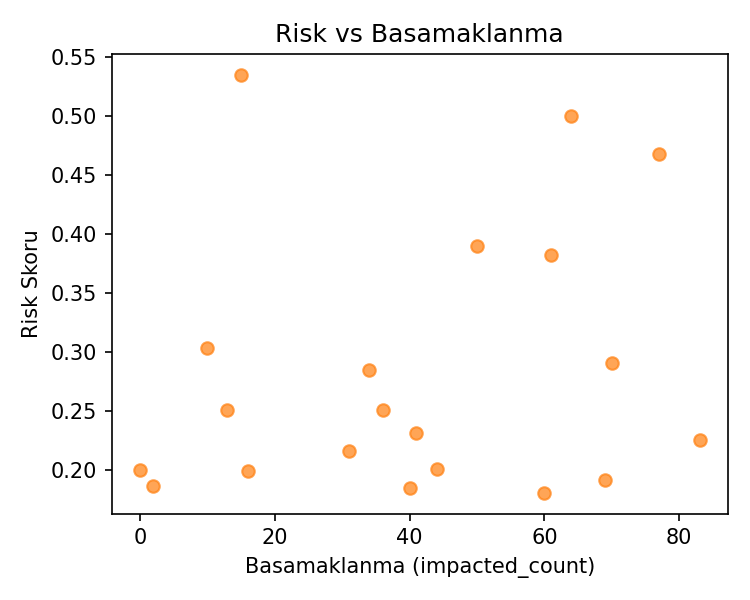
\includegraphics[width=0.6\linewidth]{../results/risk_vs_cascade.png}}{\fbox{risk\_vs\_cascade.png bulunamad\i}}
  \caption{Risk skoru ile basamaklanma etkisi aras\i ndaki ili\c{s}ki (scatter).}
\end{figure}


\section{Risk Skoru Tanımı}
Normalize edilmiş metrikler (min‑max) üzerinden ağırlıklandırılmış bir risk skoru tanımlanmıştır:
\[
\mathrm{risk}(n) = w_{in}\,\tilde{d}_{in}(n) + w_{out}\,\tilde{d}_{out}(n) + w_{b}\,\tilde{b}(n),
\]
burada $\tilde{d}_{in},\tilde{d}_{out},\tilde{b}$ sırasıyla in-degree, out-degree ve betweenness'in normalize edilmiş değerleridir. Ağırlıklar (ör. $w_{in}=0.5, w_{out}=0.2, w_{b}=0.3$) senaryoya göre ayarlanabilir.

\section{Robustluk Analizi}
Risk skoruna göre en kritik $k\in\{1,3,5\}$ düğüm kaldırıldığında zayıf bağlanırlık bileşen sayısı, en büyük bileşen boyutu ve (mümkünse) çap raporlanır. Ayrıntılar results/ dizinindeki \texttt{robustness\_risk.json} dosyasındadır.

\section{Sınırlamalar ve Gelecek Çalışmalar}
\textbf{Sınırlamalar:} (i) Varsayılan olarak yalnız \texttt{dependencies} kullanılır; \texttt{peerDependencies} isteğe bağlıdır. (ii) Betweenness hesaplaması büyük graflarda örneklemelidir; kesin değerlerin yakınsaması ağı büyüklüğüne ve $k$ seçimine bağlıdır. (iii) Global dependent sayıları doğrudan dahil edilmemiştir.

\textbf{Gelecek Çalışmalar:} (i) Global dependent metriklerinin entegrasyonu, (ii) ağırlıkların veri odaklı (öğrenilmiş) belirlenmesi, (iii) çok katmanlı ağ modelleme (örn. dev/peer/optional bağımlılık katmanları), (iv) GEXF/GraphML çıktılarıyla etkileşimli görselleştirme.

\section{Sonuç}
Bu çalışma, NPM ekosistemindeki popüler paketler için yönlü bağımlılık ağını kullanarak yapısal riskleri nicel olarak analiz etmektedir. Merkeziyet metrikleri, bileşik risk skoru ve robustluk analizleri, kritik düğümlerin ve köprülerin pratikte nasıl belirleneceğine dair net bir çerçeve sunmaktadır.

\paragraph{Çoğaltılabilirlik.} Tüm kod ve çıktı üretimi rapoyla birlikte depo içindedir. \texttt{analysis.ipynb} defteri çalıştırılarak results/ dizini yeniden üretilebilir ve bu makale \LaTeX~dosyası ile raporlanabilir.

\bibliographystyle{plain}
\begin{thebibliography}{9}
\bibitem{newman2010} Newman, M. (2010). \emph{Networks: An Introduction}. Oxford University Press.
\bibitem{brandes2001} Brandes, U. (2001). A faster algorithm for betweenness centrality. \emph{Journal of Mathematical Sociology}.
\bibitem{barabasi2016} Barabási, A.-L. (2016). \emph{Network Science}. Cambridge University Press.
\end{thebibliography}

\end{document}



